% Richard James Howe
% LaTeX Final Year Project, final report.
% Fri Apr 19 23:17:27 BST 2013
\documentclass	[a4paper, 10pt]	{article}
\usepackage	    [T1]		        {fontenc}
\usepackage	    [utf8]		      {inputenc}
\usepackage			                {lmodern}
\usepackage			                {url}
\usepackage                     {color}
\usepackage                     {hyperref}
\usepackage                     {graphicx}
\usepackage                     {placeins}
% page layout settings
% \evensidemargin	= 0pt		%default 54pt
% \textwidth	= 444pt		%default 380pt
% \hoffset	= -54pt		%default 0pt
% \topmargin	= -54pt		%default 18pt

% ===================== Settings for listings package =========================
\usepackage{listings}

\definecolor{mygreen}{rgb}{0,0.6,0}
\definecolor{mygray}{rgb}{0.5,0.5,0.5}
\definecolor{mymauve}{rgb}{0.58,0,0.82}

\lstset{ %
  backgroundcolor=\color{white},   % choose the background color; you must add \usepackage{color} or \usepackage{xcolor}
  basicstyle=\footnotesize,        % the size of the fonts that are used for the code
  breakatwhitespace=false,         % sets if automatic breaks should only happen at whitespace
  breaklines=true,                 % sets automatic line breaking
  captionpos=b,                    % sets the caption-position to bottom
  commentstyle=\color{mygreen},    % comment style
  deletekeywords={...},            % if you want to delete keywords from the given language
  escapeinside={\%*}{*)},          % if you want to add LaTeX within your code
  extendedchars=true,              % lets you use non-ASCII characters; for 8-bits encodings only, does not work with UTF-8
  frame=single,                    % adds a frame around the code
  keywordstyle=\color{blue},       % keyword style
  language=Octave,                 % the language of the code
  morekeywords={*,...},            % if you want to add more keywords to the set
  numbers=left,                    % where to put the line-numbers; possible values are (none, left, right)
  numbersep=5pt,                   % how far the line-numbers are from the code
  numberstyle=\tiny\color{mygray}, % the style that is used for the line-numbers
  rulecolor=\color{black},         % if not set, the frame-color may be changed on line-breaks within not-black text (e.g. comments (green here))
  showspaces=false,                % show spaces everywhere adding particular underscores; it overrides 'showstringspaces'
  showstringspaces=false,          % underline spaces within strings only
  showtabs=false,                  % show tabs within strings adding particular underscores
  stepnumber=2,                    % the step between two line-numbers. If it's 1, each line will be numbered
  stringstyle=\color{mymauve},     % string literal style
  tabsize=2,                       % sets default tabsize to 2 spaces
  title=\lstname                   % show the filename of files included with \lstinputlisting; also try caption instead of title
}
% ===================== Settings for listings package =========================

\newcommand*{\ditto}{---\textquotedbl---}

\newcommand{\findcite}[1]{
  \par
  \begin{center}
  \framebox[\textwidth]{
    \textcolor{red}{\emph{Find Citation on:} \textsc{#1}}
  }
  \end{center}
  \par
}

\title		{Final Year Project: A Computing System in VHDL.}
\author		{Richard James Howe}
%date		{}

\begin		{document}

	\maketitle
	\hrulefill

	\begin{abstract}
    The goal of this project is to create a computing system in VHDL from the
    ground up in order to make a product that is useful for both teaching and
    eventually much more. This project includes the firmware and the toolchain
    that is to target the device.

      \smallskip
      \begin{center}
      \noindent \textbf{Keywords}: \emph{VHDL, FORTH, SoC, CPU, Assembly.}
      \end{center}
	\end{abstract}

	\tableofcontents
  \listoffigures

  \section{Introduction}

  The idea of this project is to create an educational system for electrical
  engineers who are studying VHDL that can be eventually developed into something 
  more useful, and still have those engineers in mind. 

  This is meant to be an entire system, which is why the project spans multiple
  languages and includes different sub-projects, which can be put into roughly
  three different fields: The C/FORTH assembler program (which also finds other
  uses), the Assembler that is to run on the device and finally the VHDL that implements
  the device itself.

  I have used other peoples modules in this project and that will be clearly labelled,
  the intention was to use them and then swap them out, but some have increased
  functionality above the original goals and there were time constraints as well.

  \subsection{Contact details and licenses}

  All code, including this thesis, has been released under an open-source
  license (LGLP).

  The project is available on Github here: \url{https://github.com/howerj/fyp.git} .

  I intend to continue working on the project after university improving functionality,
  rewriting sections and porting to different devices.

  \section{Project Goals}

  The goal of this project was to create an educational computer, it was as much as
  for the education of other people as it was for me, I do not expect it to be used
  as a prototype for a real system.

  \subsection{What makes this an educational computer?}

  Nothing by itself makes this system educational, a course would have to be
  arranged around the device. 

  % Ease of use, modularity, code portability.
  % Educational computer
  %% Write assembly for the CPU
  %% Extend the system / cpu, VHDL lessons.
  %% Remove module

  \section{Tools used}
  
  As this project is entirely software based you will need a list of all the tools
  I have chosen, that will be included in this section as well as why I have used
  these tools.

    \subsection{Tools list}

    As of the $27^{th}$ of April, 2013, I have used the following to run and develop
    my project:

    \begin{itemize}
      \item Debian 6.0 (This includes a lot of the software used, eg. Gcc)
      \item Xilinx Webpack ISE 14.2 (Free for students).
      \item Git, A distributed version control system.
      \item GHDL, Digital simulation for VHDL.
      \item GTKWave, Waveform viewer.
      \item Make, For the VHDL build process.
      \item Gcc, The GNU C compiler.
      \item Bash, command interpreter.
      \item Digilent's programmer for the Nexys 3 device.
    \end{itemize}


  \section{The Hardware}
  % Nexys 3 Development board.

  The only pieces of hardware need are; a laptop, a VGA capable monitor, two micro USB cables,
  a VGA cable and Nexys 3 development board available from Digilent \cite{nexysDigilent}.

  The Nexys 3 board forms the core of this project, it is the device that I will be targeting.
  Seeing as this is an external block that is provided as is there is no real need to go into
  too many details. It provides an FPGA that has plenty of room for my project (in terms of
  Look Up Tables, Configurable Logic Blocks, Block RAMs, etcetera) as well as nice interfaces
  for external hardware (USB UART, The device can be programmed over USB, a VGA port, LEDs,
  Switches).

  The FPGA I will be using is called the XC6LX16-CS324, part of the Spartan-6 family from
  Xilinx\cite{xilinxDataSheet}. While the datasheet provides all the relevant details a
  quick overview would not go amiss. The device provides for; $12*18kB$ Block RAM (dual
  port), 32 Digital Signal Processing "slices"\footnote{A term used by Xilinx to denote
  a physical on chip device} (which includes an adder and a multiplier) and roughly
  2300 Configurable Logic Blocks (CLBs). CLBs are the bread and butter of the FPGAs,
  they are not a canonical device\footnote{Some vendors call CLBs by a different name
  but they have \emph{roughly} the same function} such as an adder or an 'OR' gate, but each FPGA is
  comprised of a version of this. An FPGA consists of an array of these devices; CLBS and
  miscellaneous other pieces of hardware such as the DSPs and BRAMs mentioned, each
  CLB has a Look Up Table (or multiple ones) which must be configured, this describes
  how the logic behaves and some flip flops for holding the internal state. These
  blocks must then be routed into something useful, the places and routing of these
  resources is a difficult problem computationally and takes up a long time.

  \findcite{CLBs, You can find out more about how they work here...}
  
  \subsection{Basic system overview}
  % Stack based machines.
  % I/O System.

      \begin{figure}[p]
        \centering
        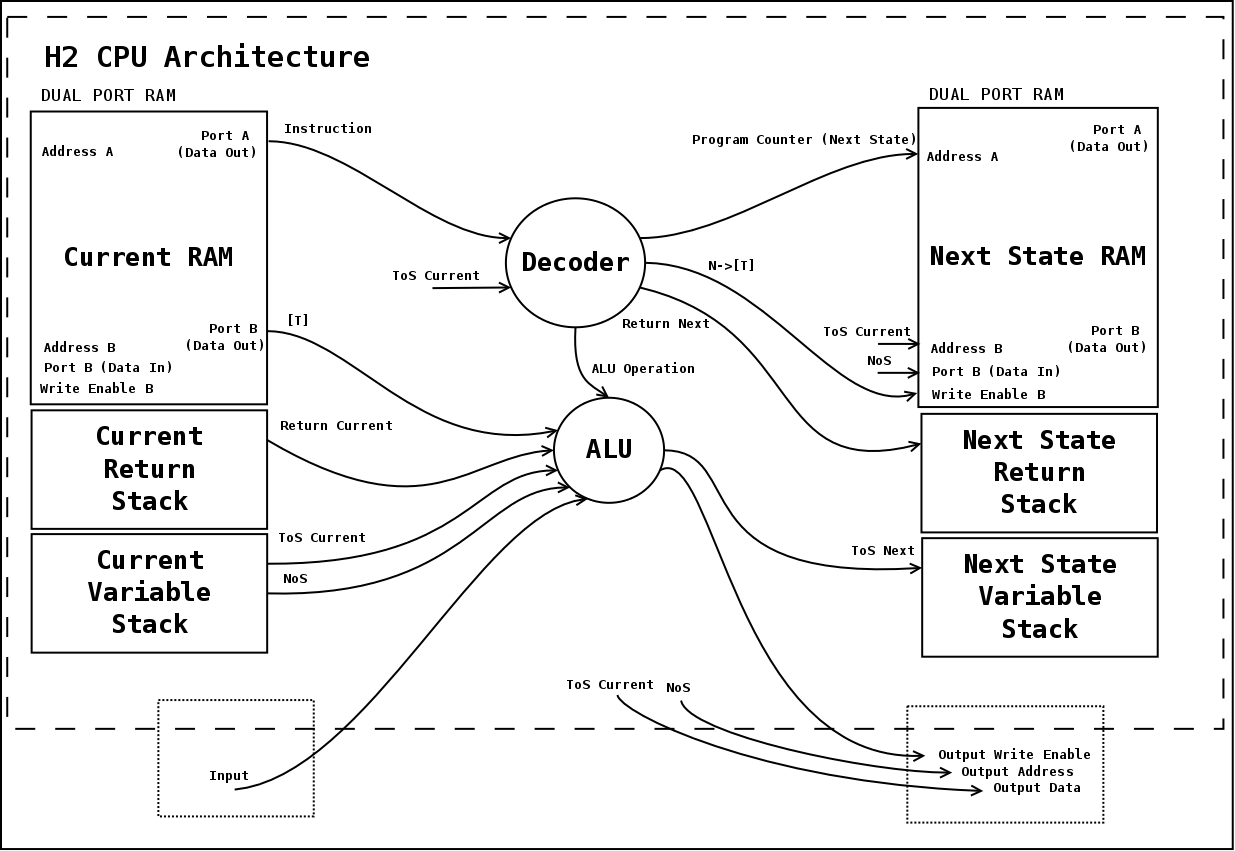
\includegraphics[width=1.1\textwidth]{pic/h2.png}
        \caption{The H2 CPU Core}
        \label{fig:H2 CPU Core}
      \end{figure}
      \FloatBarrier

  \section{VHDL}

  The main thrust of this project lies in the VHDL, all of this project revolves around
  the architecture defined here. Although most of the assembler was created separately
  as a fully blown language, the definitions for the instructions are dependant on what 
  is going on in the CPU core naturally.

    \subsection{J1}
  
    The project is built around a translation and improvement of the J1 core \cite{j1core},
    a small stack processor built in Verilog and optimized to efficiently execute FORTH
    instructions, most of which can be executed in one clock cycle. It was perfectly suited
    for my project although it was not written in my language of choice.

    \subsection{H2}

    The original core was written in Verilog, a language that lends itself to more
    compact code and where things are not as explicit, for example the exact size of
    variables.

    Getting the translation to work was fairly challenging and I also experimented with
    the core more, I moved some instructions around to allow for more ALU operations
    and added a few more instructions.

    I renamed this core the \textbf{"H2"} and it will be referred to by either this name
    or as \textbf{"CPU"} unless I say it refers to another one.

    \subsubsection{Why a stack machine?}
    \findcite{stack machines, the new wave}

    Stack machines have several advantages when it comes to embedded development compared
    to the more mainstream register machines, naturally they have disadvantages which also
    will be addressed, but they do not really apply here.

    This architecture tends to produce denser code, this is because the operands tend to
    be implicit.

    % Why stack machines?
      % Small.
      % Dense code.
      % Minimal internal state -> Fast interrupts.
      % Simpler interpreters/compilers.

    % Simple optimization Flip flops to distributed RAM.
      %% Slowed things down.
    % Multiplier.
    % Core description

    \subsubsection{The H2 Core}

    % Jump indirection.

    \subsection{VGA}
    \subsection{UART}

      The UART is the primary method of talking to the device, it is customizable at
      compile time.

    \subsection{RAM and other inferred modules}

      Instead of using Xilinx specific components you can use VHDL to create code that
      fits a certain template, this template is picked up by the synthesizer and you  
      can then verify if this is what you intended. Using this instead of instantiating
      proprietary blocks and loading the RAM with proprietary tools is a much better
      way of doing things that allows me more flexibility in how I go about things.

      The VGA unit and the CPU both have their own RAM blocks, two for the former and
      one for the latter. They are initialized from an ASCII encoded binary format,
      which while not efficient is certainly easy to process with the given tools.

      For a given file describing the RAM, for example \textbf{"h2\_mem.vhd"}, 
      the initial contents will be described in a file called \textbf{"h2\_mem.binary"}.

      All the RAM used is dual port this greatly simplifies the design, if I had to single
      port RAM I would have to worry about moving data in and out of the devices and the
      timing of it in much greater detail, it would also slow a lot of things down. For example
      the CPU would either have to adopt a Harvard architecture instead of a Von Neumann 
      or suffer a slow down.

      % Read from a file.
    \subsection{Top level}
    \subsection{Test benches and waveforms}
      % Given X show Y. Show the assembly program and the wave form that results from it.
    \subsection{Optimizations}
  \section{Build system}
    \subsection{Test benches}
    \subsection{FORTH}
    \subsection{Miscellaneous}
      % Git, make, shell.

  \section{Problems}

    There were two main problems in this project, the build time for the hardware
    implementation and the multitude of problems faced when debugging the system,
    both of which slow the project down.

    \subsection{Build time}

    Some languages like C compile fairly quickly, others provide and interactive
    environment that you can test quickly like python. Any HDL however takes
    a fairly long time to simulate and a very long time to turn this design into
    a working 'bitfile' to be uploaded to the integrated circuit. This acts as
    a friction and a drag on the development process as going from a simple change
    in a single line of code to the hardware can take upwards of fifteen minutes
    (on my computer). Simulation takes up less of that time, but it is still
    impractical to simulated even a second of real time. 

    There are a few ways
    to mitigate this, the best one is to be right the first time when you commit
    to hardware, although this can be difficult, I didn't have the time to create
    an adequate test bench to simulate incoming UART data for example, which made
    debugging the UART a slow process.

    The other simpler way is to use ever faster hardware, although that is an
    expensive option.

    \subsection{Debugging}

  \section{Documentation}

  In this section I will provide a terse (terse in the sense that this should
  be its own paper) about the system.

    \subsection{FORTH interpreter}

    Instead of being a stand alone program with only one use I decided to create
    a full blown and reusable programming language in C, the reason for the extra
    complexity is because of its utility, I have used this program not only as an
    assembler but as part of the build process in ways that are not shown in the
    code (for example for converting between file formats).

    The interpreter can trace its lineage back to an entry to the IOCCC \footnote{
    The IOCCC is the International Obfuscated C Coding Competition, the entry can
    be found here: \url{http://www.ioccc.org/all/all.tar.bz2} in the folder '1992'
    for 'buzzard.2'.}. The interpreter is drastically different from the original,
    being a complete rewrite although there are still similarities. 

    The program interprets threaded code \findcite{Threaded code} for a stack machine,
    the C program does the initial heavy lifting allowing users to interpret commands
    but it is severely lacking in capabilities initially. The trick is to write most
    of the language \emph{in itself}. This maybe odd to people coming from a background
    in a 'normal' compiled language such as C/C++ or Java. You do not modify or extend
    the language itself but instead provide new functionality via libraries you have
    written.

    Initially the language does not even have basic elements such as the "if ... else ... then"
    statements or even loops, they are written in the language itself. FORTH, and my
    dialect of it, has the ability that its syntax can be changed arbitrarily. Lets say
    you want to make an interpreter for a different language, lets say lisp, you could
    do that and start executing lisp, while at the same time it would be a valid FORTH
    program as well.

    Of note is the fact that in FORTH terminology a 'Word' does not refer to a machine
    word but instead to a defined function, so when I refer to a 'Word' I mean function.

      \subsubsection{The C Program}

      The C program itself is design to be portable being written entirely in ANSI C \findcite{
      ANSI C}, I have had this program running on my phone, and plan with some minor adjustments
      to have this running on a few embedded systems.

      The C program is a threaded code interpreter and executes something which looks
      kind of like FORTH, although there are differences. It provides methods for
      extending the language, arithmetic and logic operations, conditional jumps,
      stack manipulations, writing to/from memory and input and output functions. It
      only supplies a basic set of primitives which are:

      \begin{itemize}
        \item \textbf{":"}: Read in a word and compile a header for it in the
        dictionary, switch to \emph{compile} mode.
        \item \textbf{"immediate"}: immediate is an \emph{immediate} word which
        makes the current word under going compilation \emph{immediate}.
        \item \textbf{"read"}: Read in a space delimited word, if it is in the
        dictionary and we are in compile mode, compile a pointer in the dictionary
        to the found word, else execute it, else if it is a number push it onto
        the variable stack, else there is an error.
        \item \textbf{"$\backslash$"}: Ignore input stream until end of line 
        (ie. A comment).
        \item \textbf{"exit"}: Return from a function call.
        \item \textbf{"br"}: Branch unconditionally to address held in address
        after this instruction.
        \item \textbf{"?br"}: Same as "br" except branch conditionally when
        the top of the stack is zero.
        \item \textbf{"+"}: Pop two numbers off the variable stack, add them
        and push the result.
        \item \textbf{"-"}: \ditto Subtract them \ditto 
        \item \textbf{"*"}: \ditto Multiply them \ditto
        \item \textbf{"\%"}: Pop two numbers off the variable stack, perform
        and work out the remainder when the second item off is divided by
        the first, push the result.
        \item \textbf{"/"}: \ditto, divide the second item off by the first
        off, push the result.
        \item \textbf{"lshift"}: logical shift left the next on stack by
        first on stack places. Push the result.
        \item \textbf{"rshift"}: \ldots same but with right shift.
        \item \textbf{"and"}: Pop two numbers, compute logical conjunction of them,
        push the result.
        \item \textbf{"or"}: \ldots same but with logical disjunction.
        \item \textbf{"xor"}: \ldots same but with exclusive disjunction.
        \item \textbf{"*~*"}: Bitwise inversion of top of stack.
        \item \textbf{"1+"}: Add one to top of stack.
        \item \textbf{"1-"}: Subtract one from top of stack.
        \item \textbf{"clear"}: Clear top of stack.
        \item \textbf{"0>"}: Test if top of stack is less than zero, push result.
        \item \textbf{"="}: Pop two numbers off variable stack, test for equality,
        push result.
        \item \textbf{"<"}: Pop two items off the variable, test if the first if
        greater than the second, push the result.
        \item \textbf{">"}: \ldots same but the inverse.
        \item \textbf{"@reg"}: Use top of stack as index into the array of
        registers, push what is in there on to the variable stack.
        \item \textbf{"@dic"}: Use top of stack as index into the dictionary,
        push what is in there on to the variable stack.
        \item \textbf{"@var"}: Same but with the variable stack itself.
        \item \textbf{"@ret"}: Same but with the return stack.
        \item \textbf{"@str"}: \ldots with string storage.
        \item \textbf{"!reg"}: Store next on stack into the address pointed
        to by the first on the stack into the register file.
        \item \textbf{"!dic"}: \ldots into the dictionary.
        \item \textbf{"!var"}: \ldots into the variable stack.
        \item \textbf{"!ret"}: \ldots into the return stack.
        \item \textbf{"!str"}: \ldots into string storage.
        \item \textbf{"key"}: Push one changed from the input to the
        variable stack.
        \item \textbf{"emit"}: Pop one character from the variable stack,
        and output it.
        \item \textbf{"dup"}: Duplicate top off the variable stack.
        \item \textbf{"drop"}: Drop top of variable stack.
        \item \textbf{"swap"}: Swap top two items of variable stack.
        \item \textbf{"over"}: Duplicate the second item on the variable stack. 
        \item \textbf{">r"}: Move an item from the top of the variable
        stack to the return stack.
        \item \textbf{"r>"}: \ldots the other way around.
        \item \textbf{"tail"}: 
        \item \textbf{"'"}: Push the next compiled word onto the stack at
        run time.
        \item \textbf{","}: Advance dictionary pointer, pop the top of stack
        and write in into the dictionary.
        \item \textbf{"printnum"}: Use the top of the stack as an index into
        a string in string storage, treat this as a number and print it.
        \item \textbf{"get\_word"}: Use the top of the stack as an index into
        string storage, store a space delimited string there.
        \item \textbf{"strlen"}:
        \item \textbf{"isnumber"}:
        \item \textbf{"strnequ"}:
        \item \textbf{"\_find"}: Find a word in the dictionary if it
        exists and push a pointer to the beginning of the word header if
        it does.
        \item \textbf{"halt"}: Halt the system.
        \item \textbf{"kernel"}: Use the top of the stack to perform an
        external call. All calls have access to all the memory.
      \end{itemize}

      Also defined but not present here are three 'hidden' words, that is
      words with no name which are:

      \begin{itemize}
        \item \textbf{"Push integer"}: Pushes the next instruction onto the
        data stack, advances program counter over instruction.
        \item \textbf{"Compile"}: Compile a pointer to the execution token
        'Run' of a word.
        \item \textbf{"Run"}: Run a word, saving the return address onto the
        return stack.
      \end{itemize}

      The word ";" has not been defined here, it instead defined later like
      more of the standard words such as "rot" (rotate first three stack
      items). 

      The best documentation is the code itself, it is not too long, but
      I will give a quick overview of what happens.

      The memory is initialized, a function that is created that calls
      read then calls itself (read also handles this so the stack does
      not blow up), this forms the basic command interpreter.

      Before this is run a list of symbols is read in which forms the
      names of the initial dictionary. Then the function it has created
      is executed.

      There are two states the interpreter can be in, compile or command
      mode, in compile mode (which is what we start out in) if a word is
      found a pointer to that word is compiled into the dictionary, in
      command mode it is executed instead. There is a certain class of
      words that are always executed and they are called \emph{immediate}
      words.

      Each word compiling has the following structure:

      \begin{center}
        \begin{tabular}{l | c | c | c | r }
          \hline
          prev & str & \textbf{compile} & run & data field \ldots \\
          \hline
        \end{tabular}
      \end{center}

      Each immediate word has this structure:
      
      \begin{center}
        \begin{tabular}{l | c | c | r }
          \hline
          prev & str & \textbf{run} & data field \ldots \\
          \hline
        \end{tabular}
      \end{center}

      Where "prev" is a pointer to the previous word, "str" a pointer to the words
      name, "compile" is the instruction compile if present and "run" is the instruction
      "run". The text in bold is what is run when the word is found by "read", what makes
      the difference between an immediate and a compiling word is what is pointed to.

      The data field is of a variable length and in a normal word consists entirely or
      either pointers to other words execution field (either run or compile), numbers
      to push onto the stack or places to jump to (after either "push" or one of the
      branch instructions respectively).

      The dictionary consists of a linked list of words, and each words data field
      consists of pointers to other words making for very compact code.

      There are two stacks, a variable stack where computations are generally performed
      and a return stack for return from functions and as temporary storage. The other
      chunks of memory include a register file which contains pointers to the next
      word and instruction to execute, a pointer to the previously defined word, stack
      pointers, a pointer into the next available dictionary address as well as some
      information about the virtual machine itself. Then there is the dictionary which
      contains all the defined words as well as being used as a general storage facility.
      Finally there is a string storage space, used to store the names of words and
      other strings.

      While this description is lacking, I do have a limited space I have to write about
      each of the components so for brevities sake I will have to refer you to the
      actual code itself.
       
      \subsubsection{Basic commands and ideas}

      After the basic word list has been defined we then define more FORTH words and
      bring the interpreter/compile into a working state, loops and conditional
      statements as well as words for debugging and file operations are introduced
      here. After this the constants and system necessary for the assembler are made,
      because the assembler is still executing in the FORTH environment you can still
      call any previously defined word there.

      To interpreter is currently set up to read a start-up file, \emph{start.fs}
      which then reads the assembly file \emph{h2.fs} and outputs that to the right
      directory.

      To run the interpreter only, you would need to edit the file \emph{start.fs}
      to not run \emph{h2.fs}, which is a trivial change at the end of the file,
      just delete the lines:

      \begin{verbatim}
foutput ../vhdl/mem_h2.binary
finput h2.fs
      \end{verbatim}     
       
      You can then run the interpreter (./forth) and type 'words' to get a list of
      defined commands.

      To get a better understanding of how this interpreter works consult the
      IOCCC submission 'buzzard.2' from 1992 \cite{ioccc}

      % References to other tutorials.
      % READ, CREATE, making IF...ELSE...THEN, recursion.
    \subsection{H2 CPU}
      \subsubsection{Assembly}

   \section{Future plans}
    % More generic CPU core

    I intend to keep working on this project after I have finished university, it offers the
    potential to provide a nearly complete work bench for home use and by this you will see
    what I mean.

    There are some general improvements that could be made; making the code more uniform
    through out, adding variable stack sizes and word sizes, improving the instruction set,
    much more thorough testing (and proofs there of).

    The potential improvements here are outside the scope of the project, they were never
    intended to be included in it as I would not have had time to do so, however when I
    started the project I did have these as an eventual end goal. The platform has a lot of
    potential.

    This section fairly big despite not actually documenting the project due to the fact
    that it in part \emph{justifies} the project, this section actually more or less provides
    the reasoning for me starting the project.

    \subsection{Hardware}

      The hardware section is the one that offers the most potential when it comes to
      what can be improved with the device, although it is the section that will move
      most slowly as HDLs can be difficult to debug, more so than normal programs.

      \subsubsection{Different platforms}
        % Papilo one
      One of the goals of this project was portable of code and not just to different
      Xilinx devices either. I would like to port this system to cheaper hardware
      such as the "Papilio One". \findcite{http://papilio.cc/} This system while less
      functional costs a fraction of the Nexys 3. While the project would be more
      constrained, it should still be able to fit on the device with ease.

      I would like to get my code running on as many platforms as possible, while it
      \emph{should} be portable you can never truly find out until you have tested
      it on the real thing.

      \subsubsection{More generic code}

        If possible I would make my code as generic as I could. What I mean by this
        is being able to specify most of the parameters such as instruction size
        width and RAM size just by editing a few variables. Some of this might be
        easier than others. An example of a difficult-to-make-generic piece of code
        would be in the H2 CPU core:

        \lstset{language=VHDL,caption={Stack Depth Instruction},label=stackDepthVHDL} 
        
\begin{lstlisting}
when "01110" =>  tos_n   <=  vstkp_c & "000000" & rstkp_c; 
\end{lstlisting}

        This instruction takes two stack pointers and put them on to the stack so
        you can analyse them. However if I wanted to increase the size of the
        stack the pointers would also increase in size, taking up more room and
        rendering this instruction incorrect.

      \subsubsection{PS/2 or USB keyboard}

      A PS/2 Keyboard could be added to the board, the Nexys 3 provides a USB
      to PS/2 interface, this could be used to interact with the system instead
      of the computer.

      \subsubsection{Signal Generator}

      A signal generator should be fairly easy to design, at least internally, the
      main problem would be designing the external analogue components to work from
      ~1Hz to 100MHz (or a fraction thereof).

      The VHDL would consist of a block RAM holding the data, for example a sine wave
      or another arbitrary signal, a counter, a pointer into the memory and a few
      registers to control the device. As the RAM being used is dual port, it is
      possible to run two signals from the same RAM at a sacrifice or precision.

      This would be output in parallel over some of the boards standard I/O pins
      to a digital to analogue converter.

      \subsubsection{Data logger}

      By hooking up an external Analogue to Digital Converter (ADC) and a few other
      circuits it would be possible to have a fairly high speed data logger where
      plotting could be handled in real time on a normal computer (depending on how
      fast I manage to sample things).

      This would be the most difficult to add section and it would also be the one
      that would provide most in the way of utility.

      \subsubsection{Logic Analyser}

      With very minimal additions a logic analyser running at the speed of the device
      ($\frac{1 Sample}{Clock Cycle}$) should be attainable, the unit does not have
      to be directly controlled by the CPU core, perhaps only by setting a few registers
      to tell it how fast to sample and how much, when to begin and end and where to
      send the data.

      I can see the main problems being in where to store the data and how to get it
      off the board, I would need a faster method of communications than the UART
      unless I only intend to capture roughly 16 Kilobytes of data at a time.

      The external hardware would be quite simple, just a way to buffer and electrically
      isolate the signal from the input pins of the device.

      Instead of displaying the data on the device, it should be done instead on a
      normal desktop, at least initially.

      \subsubsection{Multiple cores}

      Due to the tiny amount of resources that are taken up by the CPU it should be
      possible to have more than on CPU core running on the platform at the same
      time, perhaps a dedicated CPU for each peripheral with one master? It would
      be a relatively easy way of increasing the power of the system.

      This is however not a priority, first increasing functionality of the base
      system by adding the aforementioned peripherals would be of greater initial
      utility, then adding more cores would be considered.

      \subsubsection{Miscellaneous}
      
      The addition of timers, the reintroduction of the multiplier and adding 
      interrupts to the new CPU core would all improve the system as a whole.

      There are also several different types of memory on the Nexys 3 board
      which could be interfaced with which would allow me to overcome the
      limitations of the H2's memory restrictions, instructions could be swapped
      in and out.

    \subsection{Firmware}

    The firmware is what could receive the most drastic improvement, getting a small
    interpreter up and running on this device is a priority. This would allow it
    to be used as a standalone system, one which I believe would be fairly useful
    to multiple people. 

    This is where the real complexity in the device would lay, eventually.

    \subsection{Build system}

    I would like to replace most of the build system with my FORTH interpreter as I
    think it would be a good show case of the language I designed, it would need
    a way for it to deal with multiple files at the same time which it currently does
    not, along with a few trivial improvements, but once that has been done I could
    use it as a replacement for all the miscellaneous shell scripts and makefiles
    that I have.

  \section{Conclusion}
    \subsection{What I would have done differently}
    \subsection{Project achievements}
  \section{References}

    \bibliographystyle{plain}              % Use plain style
    \begin{thebibliography}{1}              % Simple bibliography with widest label of 1
    \bibitem{j1core} James Bowman, Willow Garage: \emph{J1: A small Forth CPU for FPGAs},  EuroForth 2010, \url{http://www.excamera.com/files/j1.pdf} (2010)
    \bibitem{vgacore} Javier Valcarce: \emph{VHDL Macro: VGA80x40}, VHDL Monochrome VGA display adapter ,\url{http://www.javiervalcarce.eu/wiki/VHDL_Macro:_VGA80x40} (2009)
    \bibitem{uartcore} Peter Bennett: \emph{RS232 UART (VHDL)}, A UART core, \url{http://bytebash.com/2011/10/rs232-uart-vhdl/} (2012)
    \bibitem{opencore} Opencores: \emph{Open source HDL cores and code}, \url{http://opencores.org/projects} (2013)
    \bibitem{nexysDigilent} $Nexys^{TM}$3: \emph{A FPGA Spartan-6 development board}, \url{http://www.digilentinc.com/Products/Detail.cfm?NavPath=2,400,897\&Prod=NEXYS3}, (2013)
    \bibitem{ioccc} IOCCC winner Buzzard: \emph{An obfuscated FORTH interpreter}, \url{http://www.ioccc.org/1992/buzzard.2.design}, (1992)
    \bibitem{xilinxDataSheet} XC6LX16 Family Overview: \emph{Spartan-6 Family Overview}, \url{http://www.xilinx.com/support/documentation/data_sheets/ds160.pdf}, (2011)
    \end{thebibliography}



  \section{Appendix}
\end 	{document}
